\begin{figure}
	\centering
	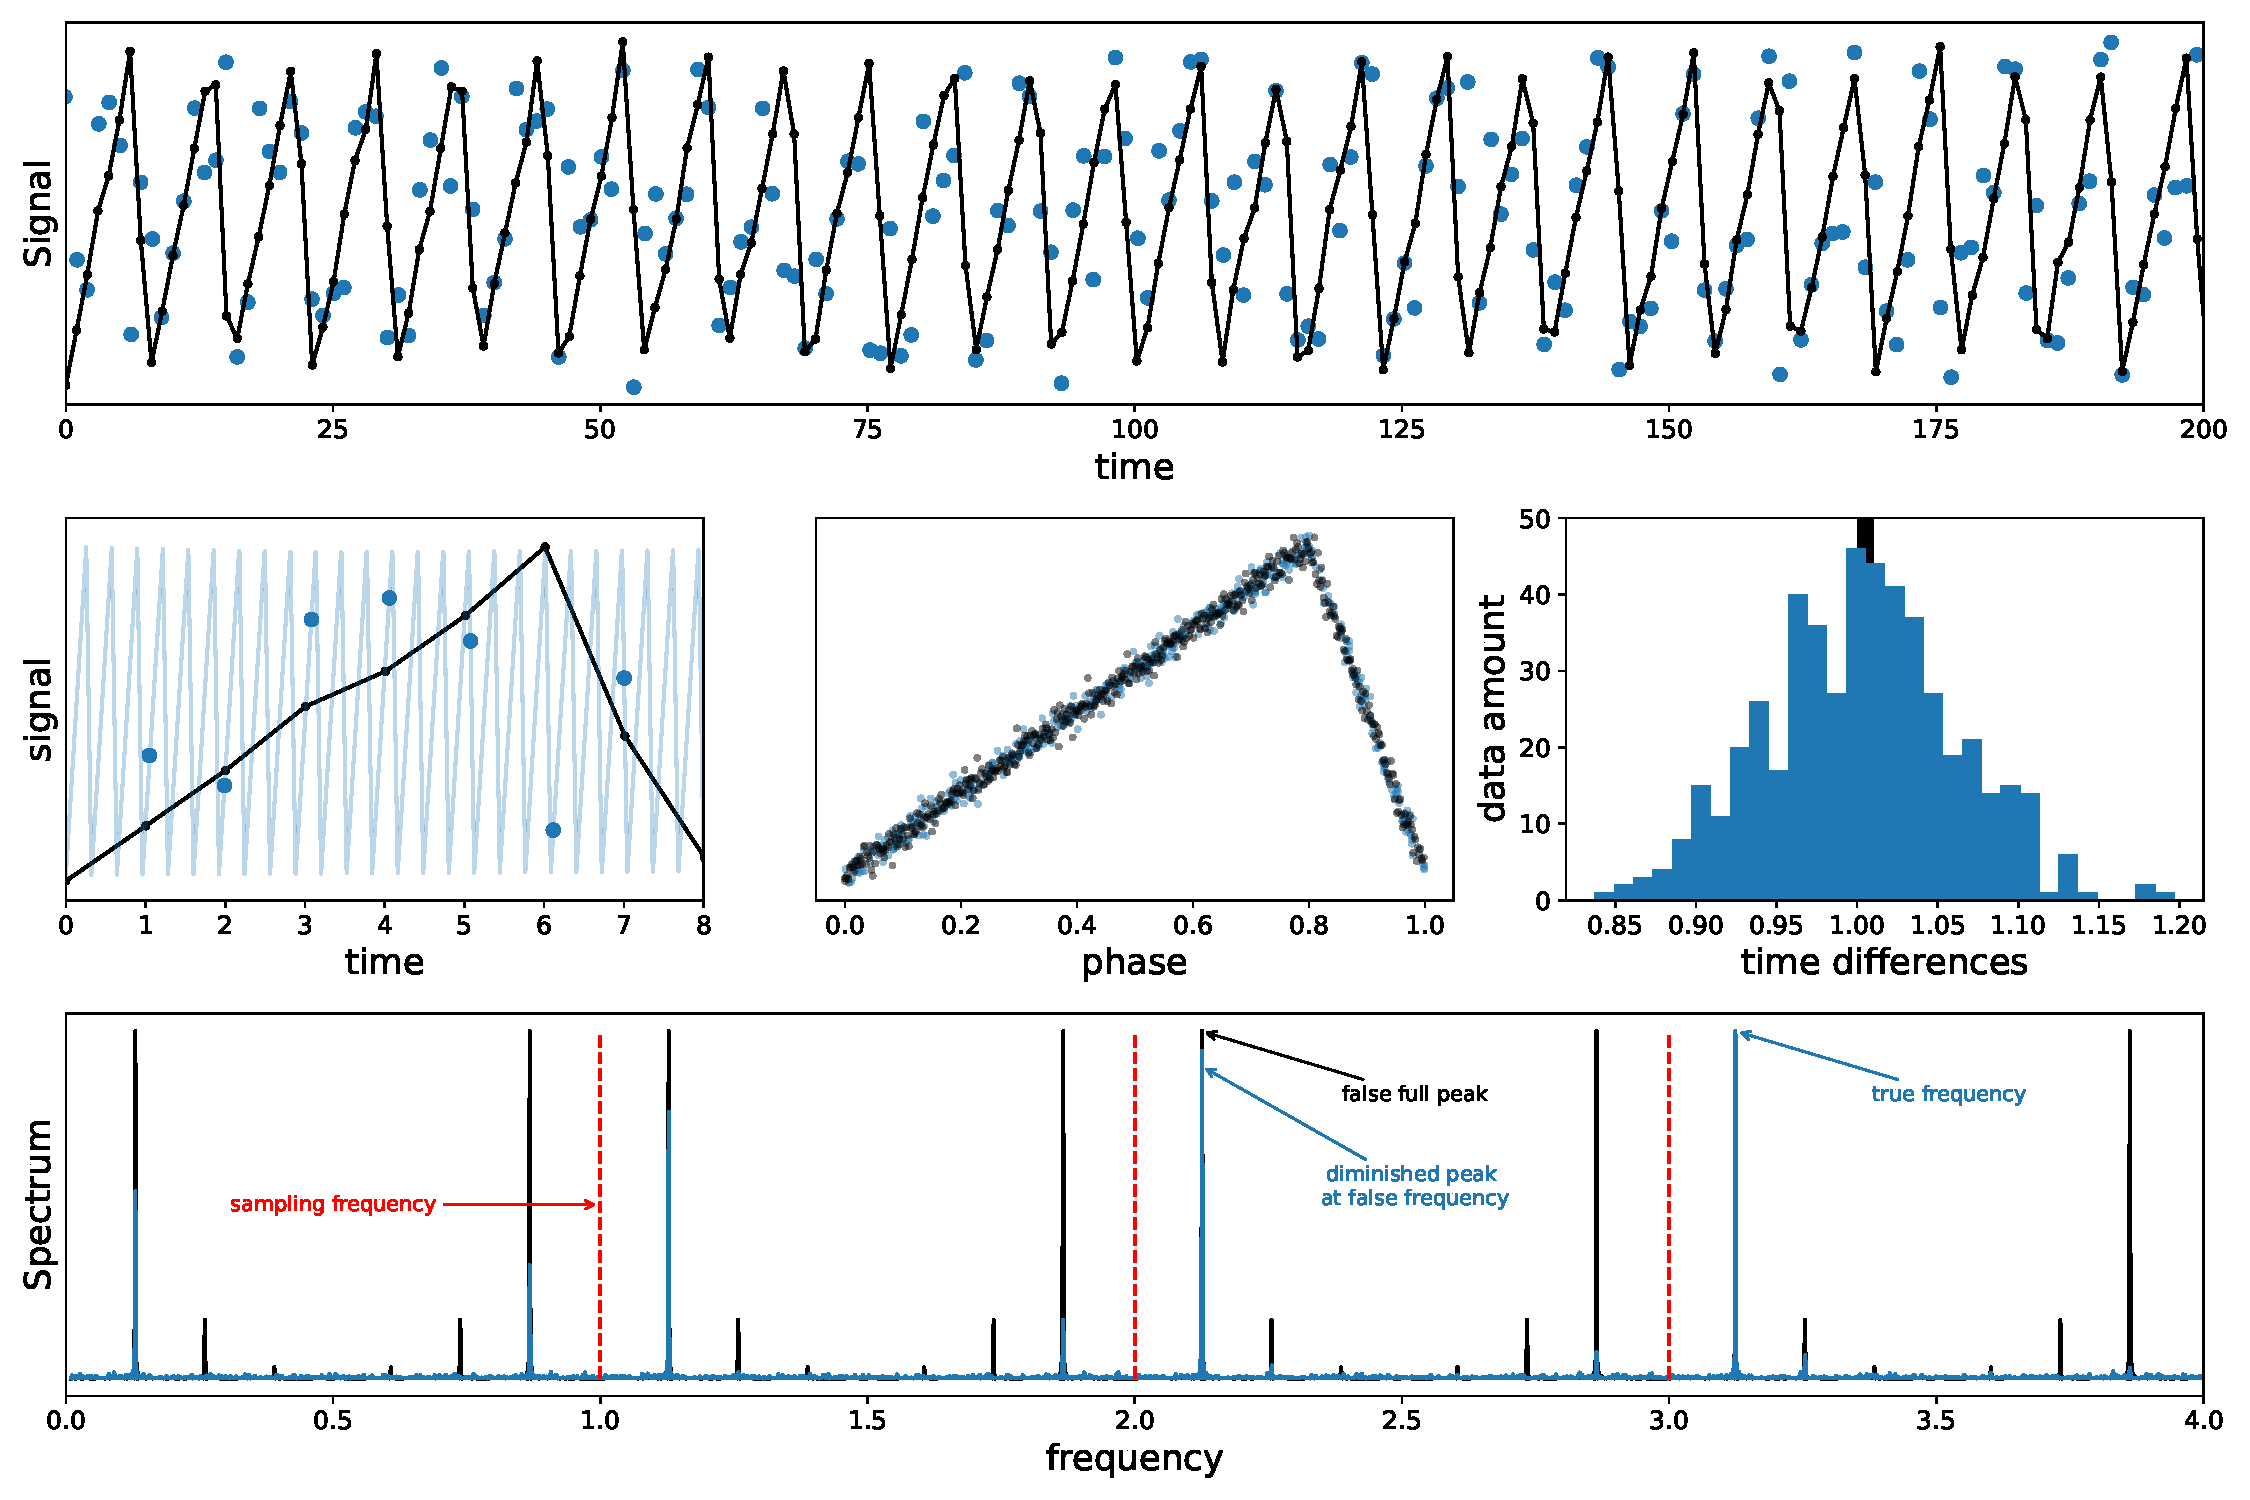
\includegraphics[width=\textwidth]{img/uneven_advantage.pdf}
	\caption[Comparison between even and uneven sampled signal past the nyquist limit]{
		Sample skewed triangular wave sampled two ways: the black dots are sampled one each unit of time.
		The sample times of the blue dots are very near one sample each unit of time, but have a litte dispersion,
		as can be seen in the left histogram.
		The frequency of the generated data is 3.124 time units.
		It is clear that the spectrum reflects every half of the sampling time (Nyquist frequency). 
		On the uneven sampling case, the spectrum does not reflect exactly; there are peaks greater than others,
		and the differences last until several times past the sampling frequency.
		The greatest peak is in the correct frequency, and the rest are partially canceled out.
		This cancellation auments with the dispersion on the sampling times, and the number of data.
		The detailed curve on the mid-left shows how exactly this happens: if the frequency is high, the dots with take an entire different path on the curve with the slightests of the temporal deviations.
	}
	\label{fig:uneven-advantage}
\end{figure}
